%!TEX root = main.tex
%Vaccine development
\begin{figure*}
    \centering
    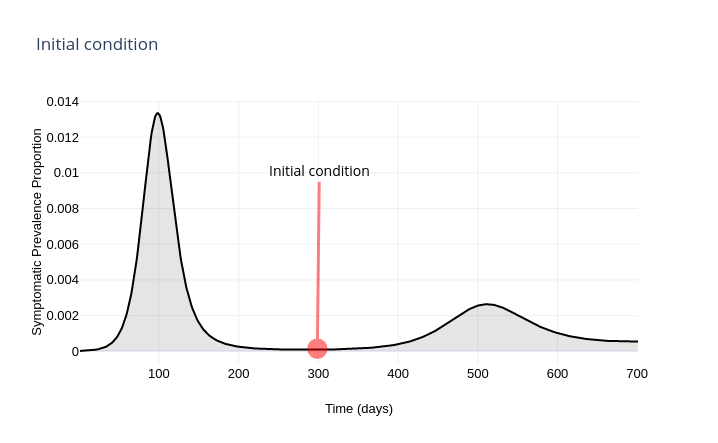
\includegraphics[scale=0.5, keepaspectratio]{figs/InitialCondition}
    \caption[Initial condition]{
        Initial condition scheme. We assume a positive prevalence. 
        For reference, at the date of write this manuscript, prevalence in CDMX 
        is around \SI{16000}{cases}, see
        \href{https://plotly.com/~sauld/36/}{https://plotly.com/~sauld/36/}
        to display an electronic viewer.}
        \label{fig:initialcondition}
\end{figure*}
\subsection{Simulation}
 According to official Governmental communication in December, Mexico treated  
\num{36000000} doses  Pfizer-Biotech, \num{76000000} doses with Aztra Seneca 
\num{18000000} quantities of Cansino-BIO. Other developments 
also are running the third Phase, and with high probability,  in the third
quarter of 2021, some of these developments will incorporate into Mexico's 
vaccine portfolio. Despite official agreements, each vaccine's delivery schedule 
is under uncertainty and-or subject to the approval of COFEPRIS.

The first accepted vaccine\textemdash Pfizer-BioNTech's BNT162b2\textemdash has 
an efficacy above \SI{90}{\percent} and requires two doses to achieve immunity. 
The other mentioned developments have a very similar profile but require 
different logistic management and stock allocation.
Thus, we face designing a dose application schedule subject to a given vaccine 
stock applied in a given period. To this end, we solve the optimal control 
problem \eqref{eqn:lockdown_vaccination_ocp}. 
We understand as solution of this problem a pair $(x(\cdot), u(\cdot))$ where
\begin{equation}
    \begin{aligned}
        x(t) &= 
            (L(t), S(t), E(t), I_S(t), I_A(t), H(t), R(t), D(t), V(t))^{\top}
        \\
        u(t) &= (u_L(t), u_V(t)) ^ {\top},
    \end{aligned}
\end{equation}
minimizes the burden of COVID-19 in DALYs \cite{WhoDALY} and the quadratic 
application cost of the lockdown-vaccination policy formulated in the functional 
\eqref{eqn:cost_functional}.  

\subsection*{Simulation Scenario}
\paragraph*{Initial Conditions}
    We assume and a hypothetical scenario where the whole population faces a 
    second wave of COVID-19. Thus whole epidemiological classes have positive 
    prevalence. We also assume that Lockdown and Susceptible compartments 
    initially enclose more than \SI{70}{\percent} of the total population, 
    and the initial prevalence of symptomatic cases is below critical levels. 
    Further, under our assumptions, the outbreaks'
    second wave implies a growth accordingly with an Effective Reproductive 
    Number (ERN) above one\textemdash Fig 10 displays a 
    qualitative schematic representation.

\begin{figure*}[tbh]
    \centering
    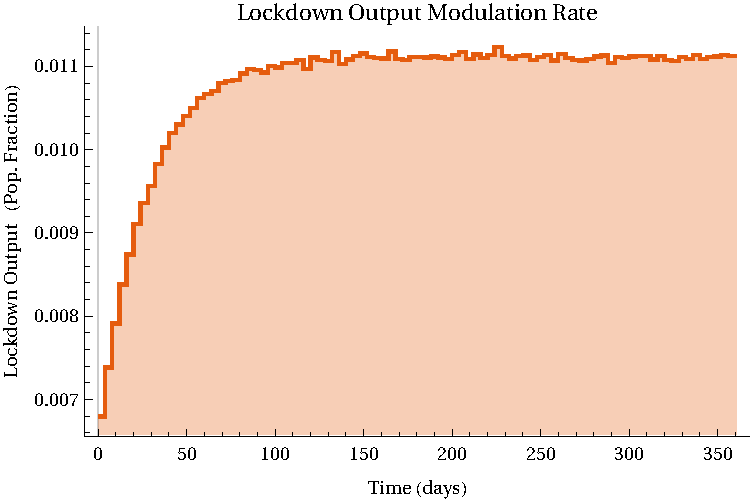
\includegraphics[width=0.7\linewidth]{figs/lockdown_control_signal}
    \caption[Lockdown modulation signal.]{Lockdown modulation signal.
    \href{https://plotly.com/~AdrianSalcedo/56/}
    {https://plotly.com/~AdrianSalcedo/56/}
            to display a electronic viewer.}
    \label{fig:lockdowncontrolsignal}
\end{figure*}

\begin{figure}
    \centering
    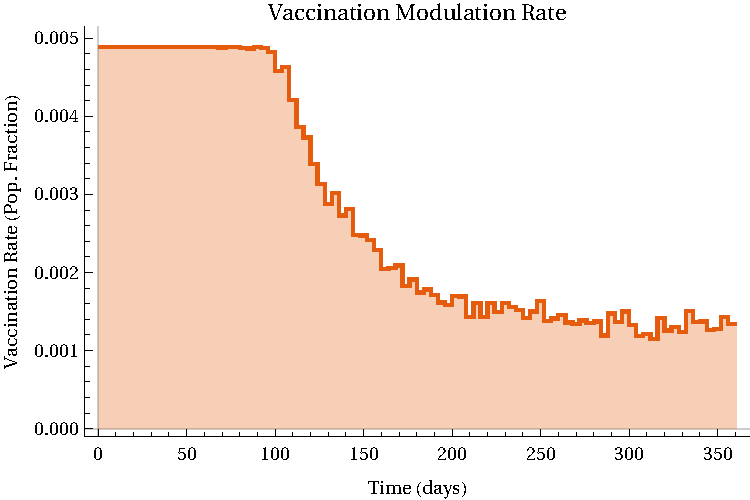
\includegraphics[width=0.7\linewidth]{figs/Vaccination_control_signal}
    \caption[Vaccination rate modulation.]{Vaccination rate modulation.
    \href{https://plotly.com/~AdrianSalcedo/58/}
    {https://plotly.com/~AdrianSalcedo/58/}}
    \label{fig:vaccinationcontrolsignal}
\end{figure}

\begin{figure}[tbh]
    \centering
    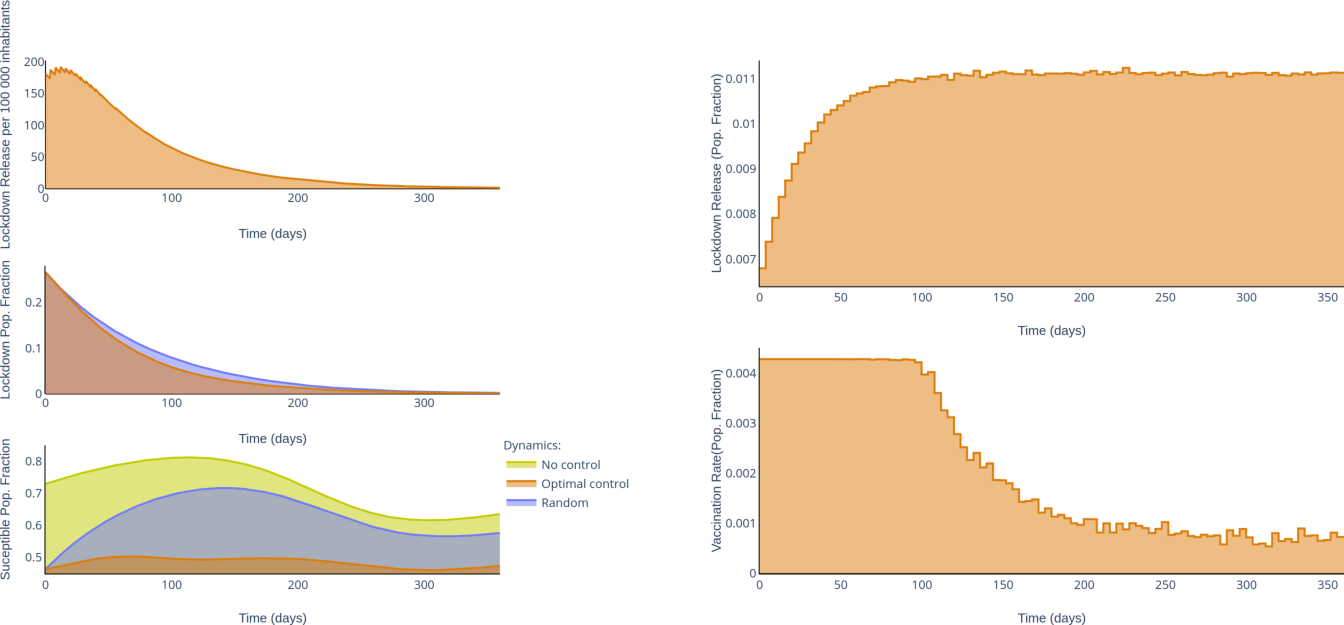
\includegraphics[scale=0.7, keepaspectratio]{%
        ./Figures/Lockdown-Release-Modulation.pdf}
    \caption{Modulation lock down release.
    \href{https://plotly.com/~AdrianSalcedo/60/}
    {https://plotly.com/~AdrianSalcedo/60/}}
    \label{fig:lockdowneffect}
\end{figure}

\begin{figure*}[tbh]
    \centering
    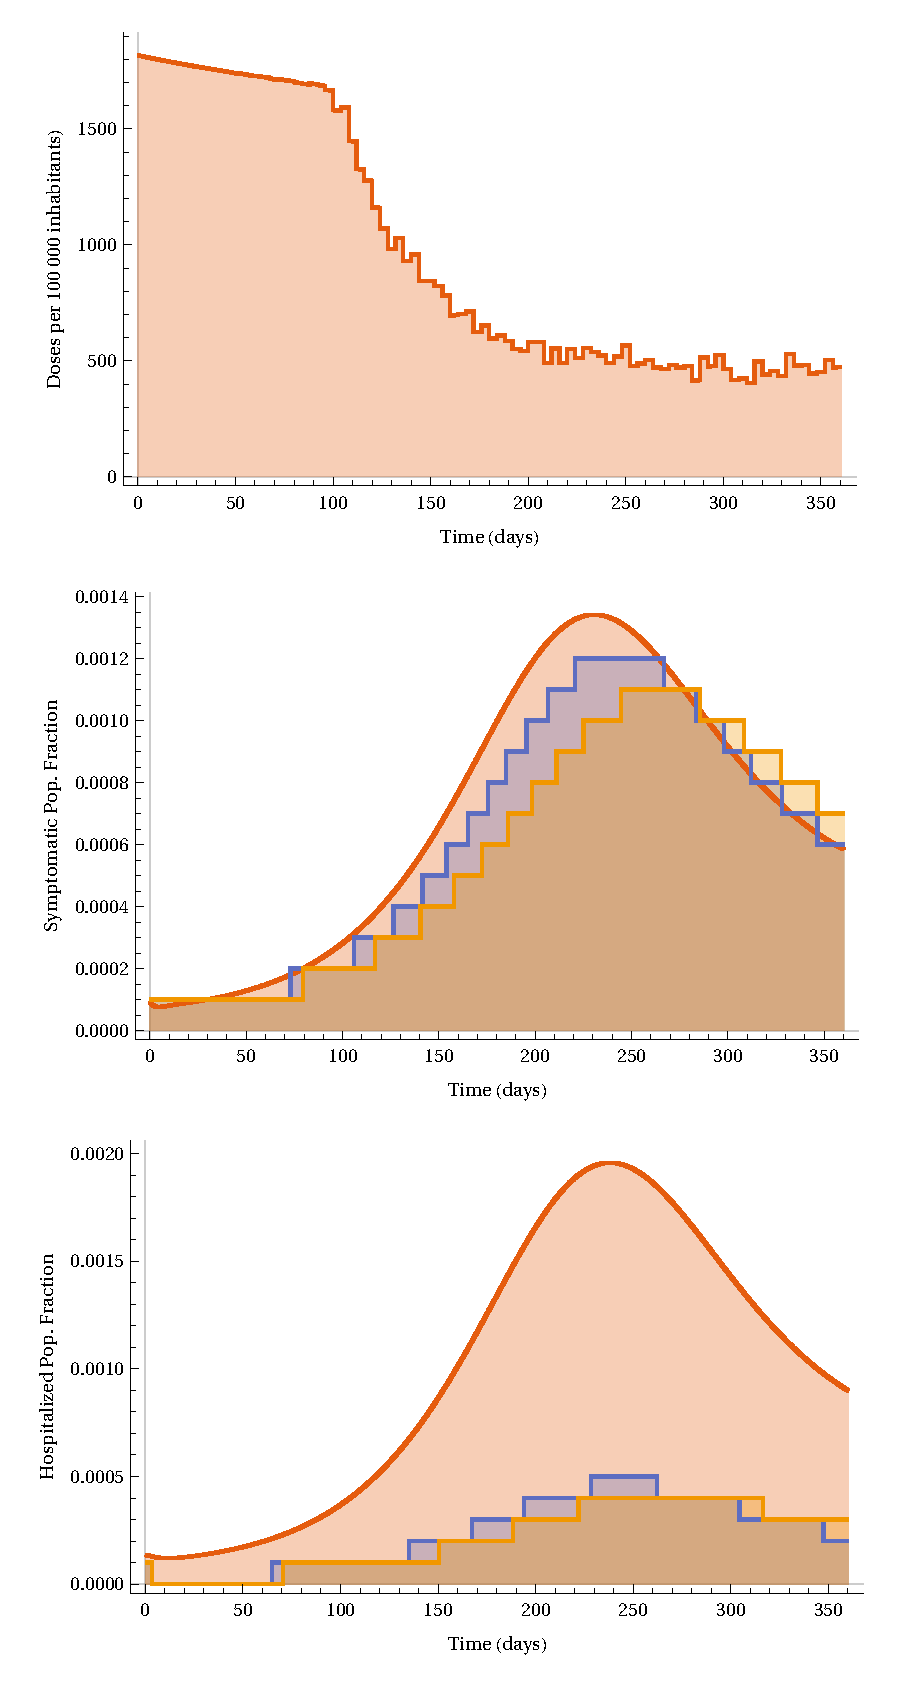
\includegraphics[scale=0.65, keepaspectratio]{figs/VaccinationEffect}
    \caption{Symptomatic Prevalence and Hozpitalization.
        \href{https://plotly.com/~AdrianSalcedo/61/}
        {https://plotly.com/~AdrianSalcedo/61/}}
    \label{fig:vaccinationeffect}
\end{figure*}
